For each network configurations during the training the rewards for each episode are recorded. Every 20000 episodes the top $95^{th}$ percentile is computed.
After each training $1000$ games are played and the highest tile is recorded in other to record if the goal of reaching the 2048 tile is achieved.

\subsection{First implementation}
In the first implementation (see \ref{lab:first_net}) the \textit{policy network} is composed by seven hidden layers fully connected and the \textit{value network} composed by four layers fully connected.
\subsubsection{First training}
$200000$ episodes:
\begin{figure}[htbp]
\centerline{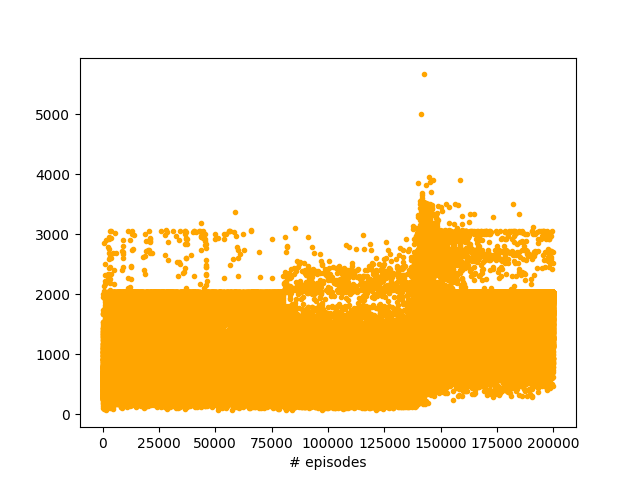
\includegraphics[scale=0.4]{05_experimental_results/05_images/ckpt-#0-1_big-net_rewards.png}}
\caption{Game score}
\label{fig:0-1_reward}
\end{figure}

\begin{figure}[htbp]
\centerline{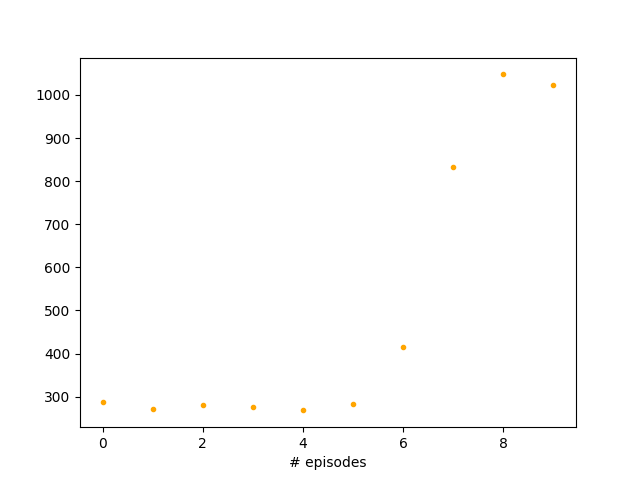
\includegraphics[scale=0.4]{05_experimental_results/05_images/ckpt-#0-1_big-net_compute_percentiles_1000_rewards.png}}
\caption{Top 95 percentile game score, computed every 20000 episodes}
\label{fig:0-1_percentile}
\end{figure}

\begin{figure}[htbp]
\centerline{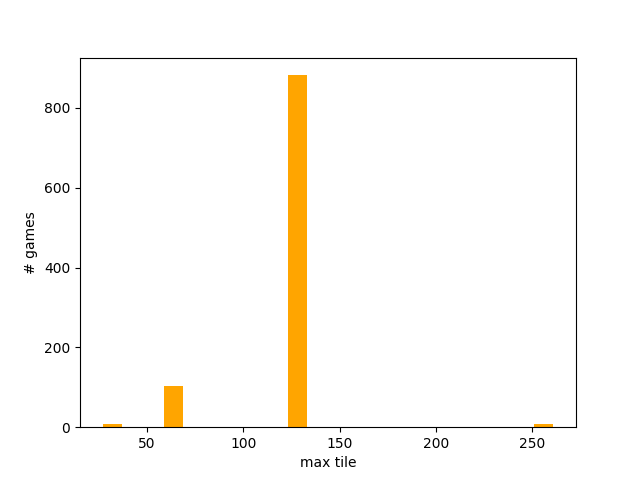
\includegraphics[scale=0.4]{05_experimental_results/05_images/ckpt-#0-1_big-net_play_games_1000_ending_states.png}}
\caption{Number of game with specific max tile's value}
\label{fig:0-1_end_state}
\end{figure}

\\
After this training, the network has learned to exhibit strategic behaviour, such as placing the highest tile in a corner and the following tiles in a diagonal pattern.
The max tile registered is in very few examples 256, still far from the goal of 2048 (fig \ref{fig:0-1_end_state}).
After $120000$ episodes, the distribution of game scores becomes more positively skewed, with a greater proportion of scores occurring at higher values (fig \ref{fig:0-1_percentile}).

\subsubsection{Second training}
$160000$ episodes using as starting board configuration $10000$ played games with probability $33\%$ (see \ref{lab:replay}):
\begin{figure}[htbp]
\centerline{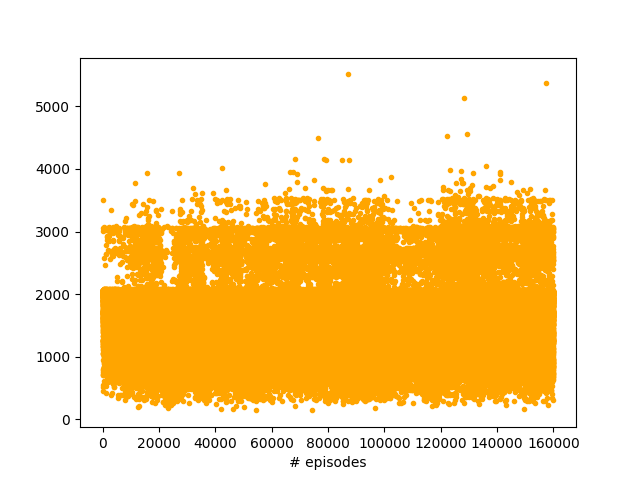
\includegraphics[scale=0.4]{05_experimental_results/05_images/ckpt-#0_big-net_replay_games_rewards.png}}
\caption{Game score}
\label{fig:0-2_reward}
\end{figure}

\begin{figure}[htbp]
\centerline{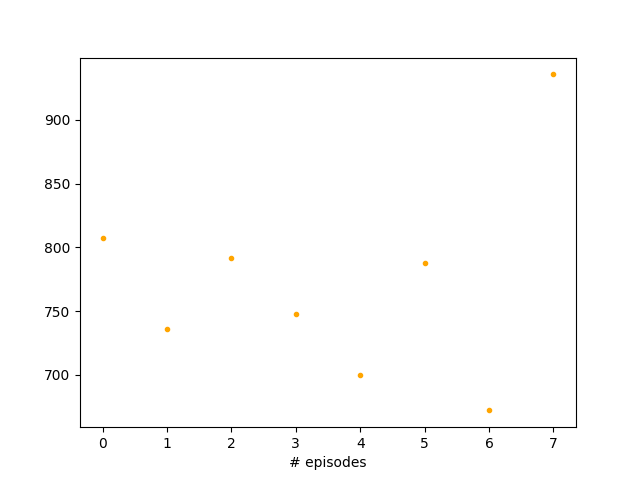
\includegraphics[scale=0.4]{05_experimental_results/05_images/ckpt-#0_big-net_replay_games_compute_percentiles_1000_rewards.png}}
\caption{Top 95 percentile game score, computed every 20000 episodes}
\label{fig:0-2_percentile}
\end{figure}

\begin{figure}[htbp]
\centerline{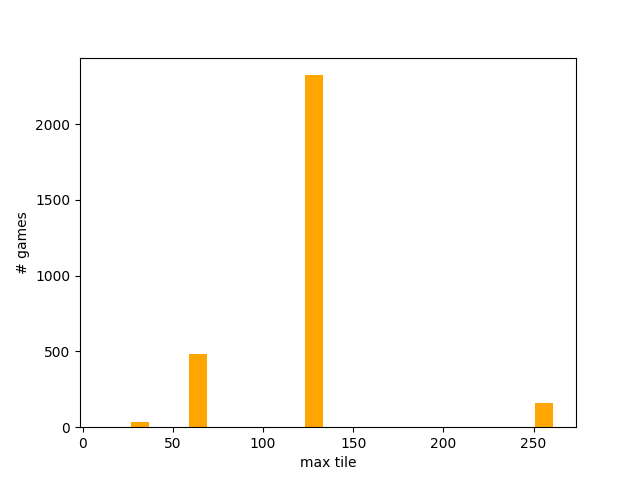
\includegraphics[scale=0.4]{05_experimental_results/05_images/ckpt-#0_big-net_replay_games_play_games_1000_ending_states.png}}
\caption{Number of game with specific max tile's value}
\label{fig:0-2_end_state}
\end{figure}

With this training the number of the 256 tiles is increased (see \ref{fig:0-2_end_state}) and the percentile value is increased (see \ref{fig:0-2_percentile}) too.

\subsection{Second implementation}
In the first implementation (see \ref{lab:second_net}) the \textit{policy network} is composed by eight hidden layers fully connected and the \textit{value network} composed by seven layers fully connected.

\subsubsection{First training}
$400000$ episodes:
\begin{figure}[htbp]
\centerline{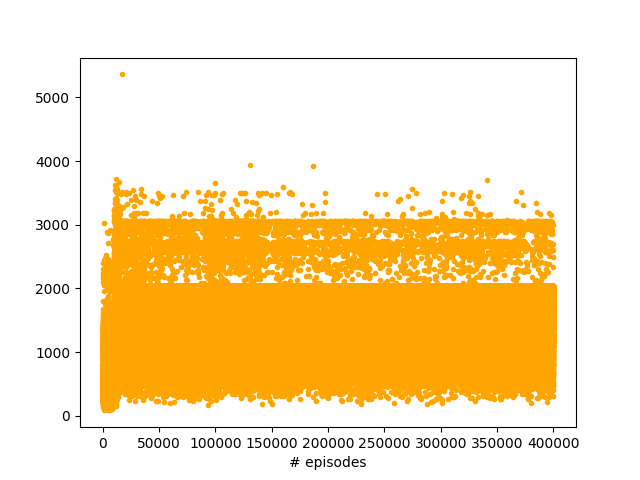
\includegraphics[scale=0.4]{05_experimental_results/05_images/ckpt-#1-0_norm_huge-net_rewards.png}}
\caption{Game score}
\label{fig:1-0_reward}
\end{figure}

\begin{figure}[htbp]
\centerline{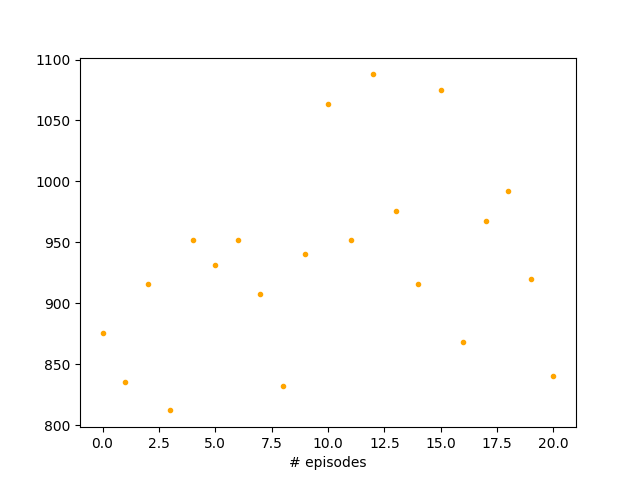
\includegraphics[scale=0.4]{05_experimental_results/05_images/ckpt-#1-0_norm_huge-net_compute_percentiles_1000_rewards.png}}
\caption{Top 95 percentile game score, computed every 20000 episodes}
\label{fig:1-0_percentile}
\end{figure}

\begin{figure}[htbp]
\centerline{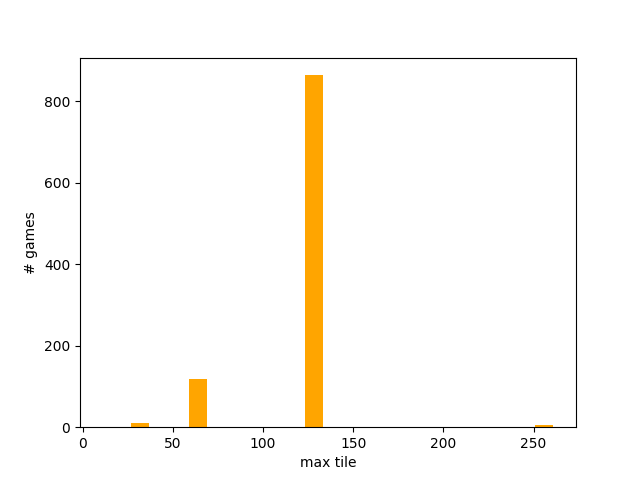
\includegraphics[scale=0.4]{05_experimental_results/05_images/ckpt-#1-0_norm_huge-net_play_games_1000_ending_states.png}}
\caption{Number of game with specific max tile's value}
\label{fig:1-0_end_state}
\end{figure}

The newly trained network exhibits better percentile values in the early episodes (fig \ref{fig:1-0_percentile}), but its performance growth rate is lower than that of the previous architecture (fig \ref{fig:0-1_percentile}).
When comparing the maximum tile plots, there are no discernible differences. However, the 128 tile is still the most prevalent (fig \ref{fig:1-0_end_state}).

\subsubsection{Second training}
$180000$ episodes using as starting board configuration $10000$ played games with probability $33\%$ (see \ref{lab:replay}):

\begin{figure}[htbp]
\centerline{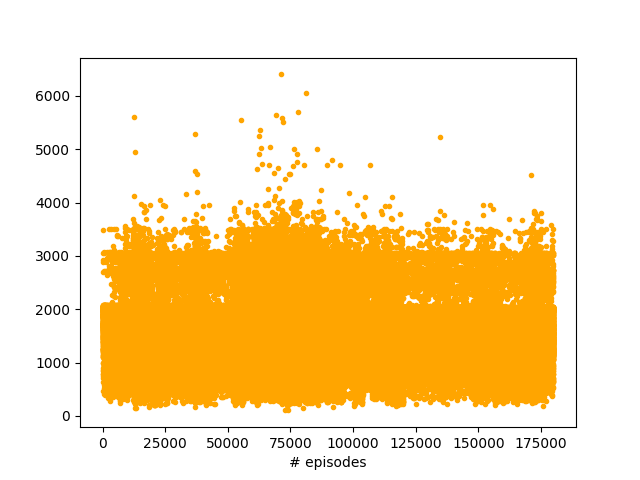
\includegraphics[scale=0.4]{05_experimental_results/05_images/ckpt-#1_big-net_replay_games_rewards.png}}
\caption{Game score}
\label{fig:1-1_reward}
\end{figure}

\begin{figure}[htbp]
\centerline{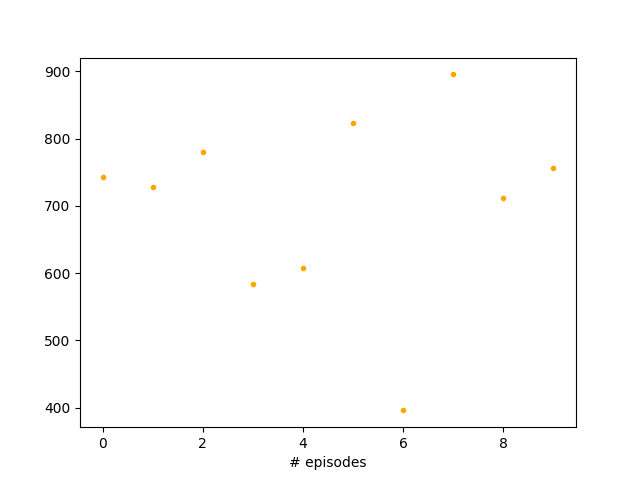
\includegraphics[scale=0.4]{05_experimental_results/05_images/ckpt-#1_big-net_replay_games_compute_percentiles_1000_rewards.png}}
\caption{Top 95 percentile game score, computed every 20000 episodes}
\label{fig:1-1_percentile}
\end{figure}

\begin{figure}[htbp]
\centerline{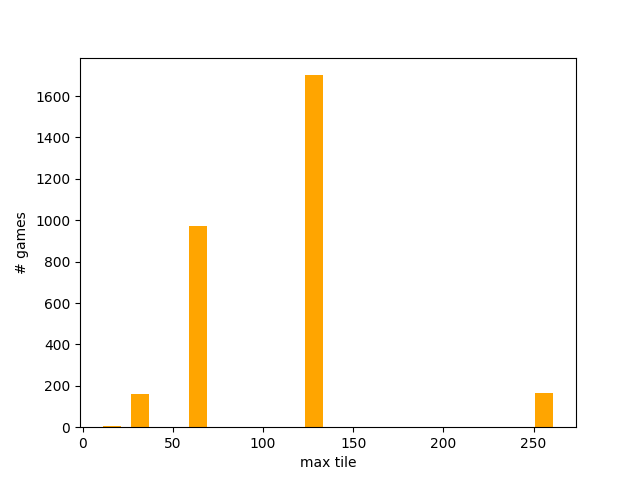
\includegraphics[scale=0.4]{05_experimental_results/05_images/ckpt-#1_big-net_replay_games_play_games_1000_ending_states.png}}
\caption{Number of game with specific max tile's value}
\label{fig:1-1_end_state}
\end{figure}

This training exhibits a substantial increase in the number of 256 tiles (fig \ref{fig:1-1_end_state}), while still maintaining the percentile values (fig \ref{fig:1-1_percentile}).